\documentclass[12pt, a4paper, oneside]{article}

\usepackage[utf8]{inputenc}
\usepackage[T1]{fontenc}
\usepackage[polish]{babel}
\usepackage{geometry}
\usepackage{graphicx}
\usepackage{booktabs}
\usepackage{array}
\usepackage{longtable}
\usepackage{hyperref}
\usepackage{float}
\usepackage{enumitem}

\geometry{margin=2.5cm}

\hypersetup{
    colorlinks=true,
    linkcolor=blue!60!black,
    urlcolor=blue!60!black
}

\raggedbottom

\begin{document}

% ============================================================
% STRONA TYTUŁOWA
% ============================================================
\begin{center}
    {\LARGE\bfseries Kamień Milowy I -- Analiza i Projekt Systemu}\\[0.8cm]
    {\Large Aplikacja do zarządzania zadaniami (Todo App)}\\[1.2cm]
    {\large Bartłomiej Karkoszka \quad Nazwisko2 \quad Nazwisko3}\\[0.3cm]
    {\large Grupa: GRUPA}\\[0.3cm]
    {\large Przedmiot: MASI}
\end{center}

\vspace{1.5cm}

% ============================================================
% 1. CEL I ZAKRES SYSTEMU
% ============================================================
\section{Cel i zakres systemu}

\subsection{Cel}
Celem systemu jest umożliwienie użytkownikom efektywnego zarządzania zadaniami osobistymi i~zespołowymi poprzez intuicyjny interfejs webowy. System pozwala na tworzenie, edycję, śledzenie postępu oraz organizację zadań z~uwzględnieniem priorytetów i~terminów realizacji.

\subsection{Zakres}
System obejmuje:
\begin{itemize}
    \item rejestrację i uwierzytelnianie użytkowników (z wykorzystaniem Keycloak),
    \item pełne operacje CRUD na zadaniach (tworzenie, odczyt, edycja, usuwanie),
    \item kategoryzację zadań według statusu (Do zrobienia, W~trakcie, Zrobione) i~priorytetu (Niski, Średni, Wysoki),
    \item widok listy zadań z filtrowaniem i wyszukiwaniem,
    \item widok tablicy Kanban z kolumnami odpowiadającymi statusom,
    \item panel główny (dashboard) z podsumowaniem statystyk zadań,
    \item przypisywanie terminów realizacji do zadań.
\end{itemize}

% ============================================================
% 2. AKTORZY SYSTEMU
% ============================================================
\section{Aktorzy systemu}

\begin{table}[H]
    \centering
    \begin{tabular}{>{\bfseries}l p{10cm}}
        \toprule
        Aktor & Opis \\
        \midrule
        Użytkownik & Osoba korzystająca z systemu -- tworzy, edytuje, przegląda i~usuwa zadania. Posiada konto w~systemie. \\[0.3cm]
        Gość & Osoba nieposiadająca konta lub niezalogowana -- może jedynie przejść do strony logowania lub rejestracji. \\[0.3cm]
        Keycloak & System zewnętrzny odpowiedzialny za uwierzytelnianie i~autoryzację użytkowników. \\
        \bottomrule
    \end{tabular}
\end{table}

% ============================================================
% 3. DIAGRAM PRZYPADKÓW UŻYCIA
% ============================================================
\section{Diagram przypadków użycia}

\begin{center}
    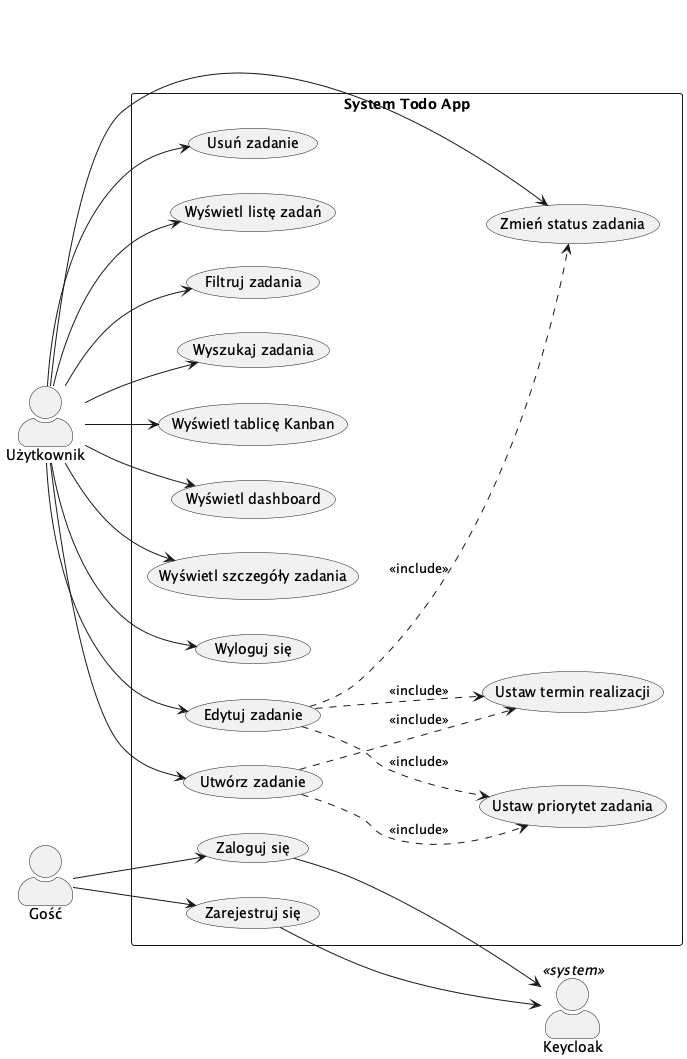
\includegraphics[width=0.9\textwidth]{diagrams/przypadki_uzycia.png}
\end{center}

Diagram przedstawia następujące przypadki użycia:
\begin{itemize}
    \item \textbf{Gość} może zalogować się lub zarejestrować (oba przypadki delegowane do Keycloak).
    \item \textbf{Użytkownik} po zalogowaniu ma dostęp do pełnej funkcjonalności: zarządzania zadaniami, filtrowania, wyszukiwania, widoku Kanban i dashboardu.
    \item Tworzenie i edycja zadania zawierają (\texttt{<<include>>}) ustawianie priorytetu i~terminu realizacji.
\end{itemize}

% ============================================================
% 4. WYMAGANIA FUNKCJONALNE
% ============================================================
\section{Wymagania funkcjonalne}

\begin{longtable}{p{11cm} l}
    \toprule
    \textbf{Wymaganie} & \textbf{Priorytet} \\
    \midrule
    \endfirsthead
    \toprule
    \textbf{Wymaganie} & \textbf{Priorytet} \\
    \midrule
    \endhead
    System umożliwia rejestrację nowego użytkownika poprzez Keycloak & Wysoki \\[0.15cm]
    System umożliwia logowanie użytkownika poprzez Keycloak & Wysoki \\[0.15cm]
    System umożliwia wylogowanie użytkownika & Wysoki \\[0.15cm]
    System umożliwia tworzenie nowego zadania z~tytułem, opisem, priorytetem i~terminem realizacji & Wysoki \\[0.15cm]
    System umożliwia edycję istniejącego zadania & Wysoki \\[0.15cm]
    System umożliwia usuwanie zadania & Wysoki \\[0.15cm]
    System umożliwia wyświetlanie listy wszystkich zadań użytkownika & Wysoki \\[0.15cm]
    System umożliwia filtrowanie zadań według statusu (TODO, IN\_PROGRESS, DONE) & Średni \\[0.15cm]
    System umożliwia filtrowanie zadań według priorytetu (LOW, MEDIUM, HIGH) & Średni \\[0.15cm]
    System umożliwia wyszukiwanie zadań po tytule/słowie kluczowym & Średni \\[0.15cm]
    System wyświetla tablicę Kanban z~kolumnami odpowiadającymi statusom zadań & Średni \\[0.15cm]
    System wyświetla panel dashboard z~podsumowaniem liczby zadań w~poszczególnych statusach & Niski \\[0.15cm]
    System umożliwia zmianę statusu zadania & Wysoki \\[0.15cm]
    System umożliwia przypisanie priorytetu do zadania & Wysoki \\[0.15cm]
    System umożliwia ustawienie terminu realizacji zadania & Średni \\
    \bottomrule
\end{longtable}

% ============================================================
% 5. WYMAGANIA NIEFUNKCJONALNE
% ============================================================
\section{Wymagania niefunkcjonalne}

\begin{longtable}{p{11cm} l}
    \toprule
    \textbf{Wymaganie} & \textbf{Kategoria} \\
    \midrule
    \endfirsthead
    \toprule
    \textbf{Wymaganie} & \textbf{Kategoria} \\
    \midrule
    \endhead
    Interfejs użytkownika musi być responsywny (desktop, tablet, mobile) & Użyteczność \\[0.15cm]
    System musi obsługiwać przeglądarki Chrome, Firefox i~Safari w~najnowszych wersjach & Kompatybilność \\[0.15cm]
    Czas odpowiedzi API nie powinien przekraczać 500ms dla operacji CRUD & Wydajność \\[0.15cm]
    System musi wykorzystywać HTTPS do komunikacji klient--serwer & Bezpieczeństwo \\[0.15cm]
    Uwierzytelnianie musi być realizowane przez zewnętrzny serwer Keycloak (OAuth2/OpenID Connect) & Bezpieczeństwo \\[0.15cm]
    Hasła użytkowników nie są przechowywane bezpośrednio w~systemie (delegacja do Keycloak) & Bezpieczeństwo \\[0.15cm]
    Frontend musi być zbudowany w~oparciu o~React~19 z~TypeScript & Technologia \\[0.15cm]
    Backend musi udostępniać REST API & Technologia \\[0.15cm]
    Dane muszą być przechowywane w~relacyjnej bazie danych (PostgreSQL) & Technologia \\[0.15cm]
    System powinien być łatwo wdrażalny za pomocą kontenerów Docker & Wdrożenie \\[0.15cm]
    Kod źródłowy musi być wersjonowany w~repozytorium Git & Utrzymanie \\[0.15cm]
    System powinien obsługiwać jednocześnie co najmniej 50~użytkowników & Wydajność \\
    \bottomrule
\end{longtable}

% ============================================================
% 6. WSTĘPNY DIAGRAM KLAS
% ============================================================
\clearpage
\section{Wstępny diagram klas}

\begin{center}
    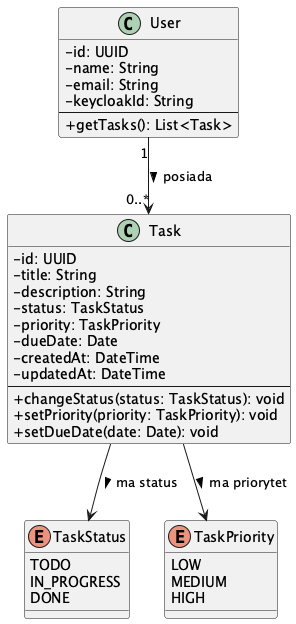
\includegraphics[width=0.65\textwidth]{diagrams/diagram_klas.png}
\end{center}

Model dziedziny obejmuje następujące klasy:
\begin{itemize}
    \item \textbf{User} -- reprezentuje użytkownika systemu, powiązanego z~Keycloak poprzez pole \texttt{keycloakId}.
    \item \textbf{Task} -- podstawowa encja systemu, zawierająca tytuł, opis, status, priorytet, termin realizacji oraz znaczniki czasowe.
    \item \textbf{TaskStatus} -- typ wyliczeniowy definiujący stany zadania: \texttt{TODO}, \texttt{IN\_PROGRESS}, \texttt{DONE}.
    \item \textbf{TaskPriority} -- typ wyliczeniowy definiujący priorytety: \texttt{LOW}, \texttt{MEDIUM}, \texttt{HIGH}.
\end{itemize}

Relacja: jeden użytkownik posiada wiele zadań (1 do 0..*).

% ============================================================
% 7. WSTĘPNY DIAGRAM KOMPONENTÓW
% ============================================================
\section{Wstępny diagram komponentów}

\begin{center}
    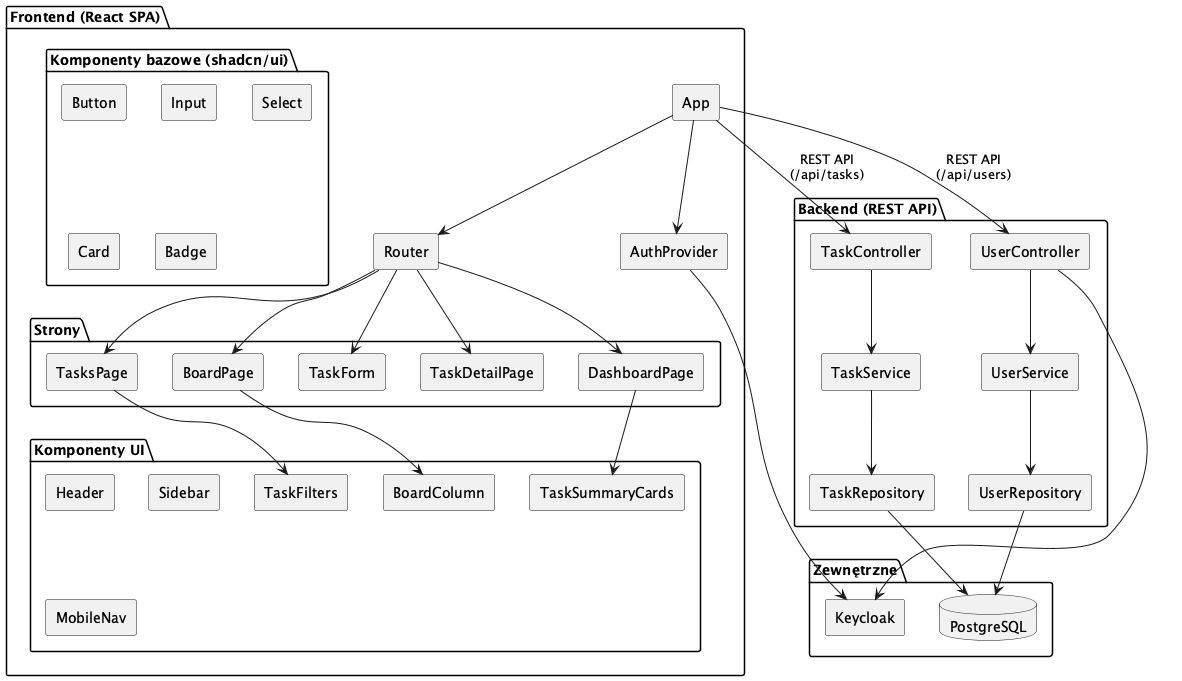
\includegraphics[width=\textwidth]{diagrams/diagram_komponentow.png}
\end{center}

System składa się z trzech głównych pakietów:
\begin{itemize}
    \item \textbf{Frontend (React SPA)} -- aplikacja kliencka zawierająca strony (Dashboard, Tasks, Board), komponenty UI (Header, Sidebar, filtry) oraz komponenty bazowe (shadcn/ui).
    \item \textbf{Backend (REST API)} -- warstwa serwerowa z kontrolerami, serwisami i~repozytoriami obsługującymi logikę biznesową.
    \item \textbf{Systemy zewnętrzne} -- baza danych PostgreSQL oraz serwer uwierzytelniania Keycloak.
\end{itemize}

Komunikacja między frontendem a backendem odbywa się przez REST API pod ścieżkami \texttt{/api/tasks} i~\texttt{/api/users}.

% ============================================================
% 8. WSTĘPNY DIAGRAM WARSTW SYSTEMU
% ============================================================
\section{Wstępny diagram warstw systemu}

\begin{center}
    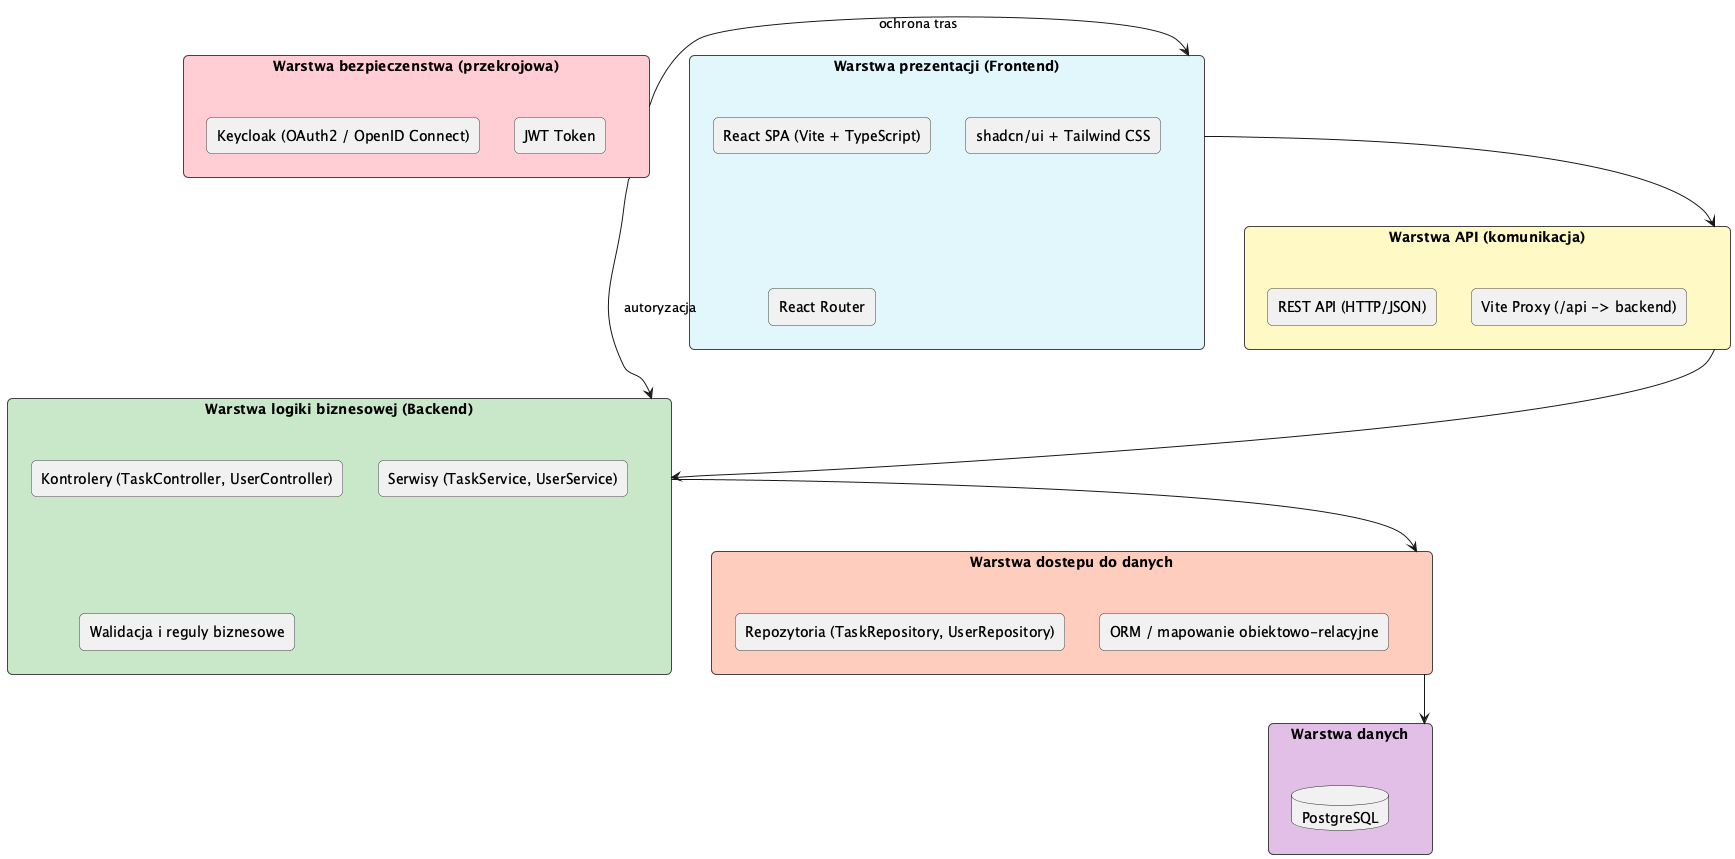
\includegraphics[width=0.75\textwidth]{diagrams/diagram_warstw.png}
\end{center}

Architektura systemu oparta jest na modelu warstwowym:
\begin{enumerate}
    \item \textbf{Warstwa prezentacji} -- aplikacja React SPA z~Tailwind CSS i~React Router.
    \item \textbf{Warstwa API} -- komunikacja REST (HTTP/JSON) między frontendem a backendem, z~wykorzystaniem proxy Vite w~trybie deweloperskim.
    \item \textbf{Warstwa logiki biznesowej} -- kontrolery, serwisy oraz reguły walidacji.
    \item \textbf{Warstwa dostępu do danych} -- repozytoria i~mapowanie obiektowo-relacyjne (ORM).
    \item \textbf{Warstwa danych} -- relacyjna baza danych PostgreSQL.
\end{enumerate}

Warstwa bezpieczeństwa (Keycloak, tokeny JWT) jest warstwą przekrojową, przenikającą zarówno warstwę prezentacji (ochrona tras), jak i~warstwę logiki biznesowej (autoryzacja żądań).

% ============================================================
% 9. SŁOWNIK POJĘĆ
% ============================================================
\section{Słownik pojęć}

\begin{table}[H]
    \centering
    \begin{tabular}{>{\bfseries}l p{10cm}}
        \toprule
        Pojęcie & Definicja \\
        \midrule
        Zadanie (Task) & Podstawowa jednostka pracy w~systemie, posiadająca tytuł, opis, status, priorytet i~termin realizacji. \\[0.2cm]
        Status & Stan realizacji zadania: Do zrobienia (TODO), W~trakcie (IN\_PROGRESS), Zrobione (DONE). \\[0.2cm]
        Priorytet & Poziom ważności zadania: Niski (LOW), Średni (MEDIUM), Wysoki (HIGH). \\[0.2cm]
        Tablica Kanban & Wizualizacja zadań w~kolumnach odpowiadających statusom. \\[0.2cm]
        Dashboard & Panel główny z~podsumowaniem statystyk zadań użytkownika. \\
        \bottomrule
    \end{tabular}
\end{table}

% ============================================================
% 10. STOS TECHNOLOGICZNY
% ============================================================
\section{Stos technologiczny}

\begin{table}[H]
    \centering
    \begin{tabular}{>{\bfseries}l p{10cm}}
        \toprule
        Warstwa & Technologia \\
        \midrule
        Frontend & React 19, TypeScript, Vite, Tailwind CSS v4, shadcn/ui, React Router v7 \\
        Backend & Spring Boot (Java) lub Go -- w~trakcie decyzji \\
        Baza danych & PostgreSQL \\
        Uwierzytelnianie & Keycloak (OAuth2 / OpenID Connect) \\
        Konteneryzacja & Docker, Docker Compose \\
        Kontrola wersji & Git \\
        \bottomrule
    \end{tabular}
\end{table}

\end{document}
